%!TeX root=../pridetop.tex
\chapter[Chapter \thechapter]{}
	
	
\begin{figure}[t!]
\centering

\includegraphics[width=\linewidth]{54top}
\captionlistentry{Jane happened to look round}
\end{figure}


\lettrine[lines=6,image=true]{initials/chap54a}{s}  soon as they were gone, Elizabeth walked out to recover her spirits; or, in other words, to dwell without interruption on those subjects which must deaden them more. Mr Darcy's behaviour astonished and vexed her.

\zz
»Why, if he came only to be silent, grave, and indifferent,« said she, »did he come at all?«

She could settle it in no way that gave her pleasure.

»He could be still amiable, still pleasing to my uncle and aunt, when he was in town; and why not to me? If he fears me, why come hither? If he no longer cares for me, why silent? Teasing, teasing man! I will think no more about him.«

Her resolution was for a short time involuntarily kept by the approach of her sister, who joined her with a cheerful look which showed her better satisfied with their visitors than Elizabeth.

»Now,« said she, »that this first meeting is over, I feel perfectly easy. I know my own strength, and I shall never be embarrassed again by his coming. I am glad he dines here on Tuesday. It will then be publicly seen, that on both sides we meet only as common and indifferent acquaintance.«

»Yes, very indifferent, indeed,« said Elizabeth, laughingly. »Oh, Jane! take care.«

»My dear Lizzy, you cannot think me so weak as to be in danger now.«

»I think you are in very great danger of making him as much in love with you as ever.«

They did not see the gentlemen again till Tuesday; and Mrs Bennet, in the meanwhile, was giving way to all the happy schemes which the good-humour and common politeness of Bingley, in half an hour's visit, had revived.

On Tuesday there was a large party assembled at Longbourn; and the two who were most anxiously expected, to the credit of their punctuality as sportsmen, were in very good time. When they repaired to the dining-room, Elizabeth eagerly watched to see whether Bingley would take the place which, in all their former parties, had belonged to him, by her sister. Her prudent mother, occupied by the same ideas, forbore to invite him to sit by herself. On entering the room, he seemed to hesitate; but Jane happened to look round, and happened to smile: it was decided. He placed himself by her.

Elizabeth, with a triumphant sensation, looked towards his friend. He bore it with noble indifference; and she would have imagined that Bingley had received his sanction to be happy, had she not seen his eyes likewise turned towards Mr Darcy, with an expression of half-laughing alarm.

His behaviour to her sister was such during dinnertime as showed an admiration of her, which, though more guarded than formerly, persuaded Elizabeth, that, if left wholly to himself, Jane's happiness, and his own, would be speedily secured. Though she dared not depend upon the consequence, she yet received pleasure from observing his behaviour. It gave her all the animation that her spirits could boast; for she was in no cheerful humour. Mr Darcy was almost as far from her as the table could divide them. He was on one side of her mother. She knew how little such a situation would give pleasure to either, or make either appear to advantage. She was not near enough to hear any of their discourse; but she could see how seldom they spoke to each other, and how formal and cold was their manner whenever they did. Her mother's ungraciousness made the sense of what they owed him more painful to Elizabeth's mind; and she would, at times, have given anything to be privileged to tell him, that his kindness was neither unknown nor unfelt by the whole of the family.

She was in hopes that the evening would afford some opportunity of bringing them together; that the whole of the visit would not pass away without enabling them to enter into something more of conversation, than the mere ceremonious salutation attending his entrance. Anxious and uneasy, the period which passed in the drawing-room before the gentlemen came, was wearisome and dull to a degree that almost made her uncivil. She looked forward to their entrance as the point on which all her chance of pleasure for the evening must depend.

»If he does not come to me, \textit{then},« said she, »I shall give him up for ever.«

The gentlemen came; and she thought he looked as if he would have answered her hopes; but, alas! the ladies had crowded round the table, where Miss Bennet was making tea, and Elizabeth pouring out the coffee, in so close a confederacy, that there was not a single vacancy near her which would admit of a chair. And on the gentlemen's approaching, one of the girls moved closer to her than ever, and said, in a whisper,—

»The men shan't come and part us, I am determined. We want none of them; do we?«

Darcy had walked away to another part of the room. She followed him with her eyes, envied everyone to whom he spoke, had scarcely patience enough to help anybody to coffee, and then was enraged against herself for being so silly!

»A man who has once been refused! How could I ever be foolish enough to expect a renewal of his love? Is there one among the sex who would not protest against such a weakness as a second proposal to the same woman? There is no indignity so abhorrent to their feelings.«

She was a little revived, however, by his bringing back his coffee-cup himself; and she seized the opportunity of saying,—

»Is your sister at Pemberley still?«

»Yes; she will remain there till Christmas.«

»And quite alone? Have all her friends left her?«

»Mrs Annesley is with her. The others have been gone on to Scarborough these three weeks.«

She could think of nothing more to say; but if he wished to converse with her, he might have better success. He stood by her, however, for some minutes, in silence; and, at last, on the young lady's whispering to Elizabeth again, he walked away.

When the tea things were removed, and the card tables placed, the ladies all rose; and Elizabeth was then hoping to be soon joined by him, when all her views were overthrown, by seeing him fall a victim to her mother's rapacity for whist players, and in a few moments after seated with the rest of the party. She now lost every expectation of pleasure. They were confined for the evening at different tables; and she had nothing to hope, but that his eyes were so often turned towards her side of the room, as to make him play as unsuccessfully as herself.

Mrs Bennet had designed to keep the two Netherfield gentlemen to supper; but their carriage was, unluckily, ordered before any of the others, and she had no opportunity of detaining them.

»Well, girls,« said she, as soon as they were left to themselves, »what say you to the day? I think everything has passed off uncommonly well, I assure you. The dinner was as well dressed as any I ever saw. The venison was roasted to a turn—and everybody said, they never saw so fat a haunch. The soup was fifty times better than what we had at the Lucases' last week; and even Mr Darcy acknowledged that the partridges were remarkably well done; and I suppose he has two or three French cooks at least. And, my dear Jane, I never saw you look in greater beauty. Mrs Long said so too, for I asked her whether you did not. And what do you think she said besides? »Ah! Mrs Bennet, we shall have her at Netherfield at last!« She did, indeed. I do think Mrs Long is as good a creature as ever lived—and her nieces are very pretty behaved girls, and not at all handsome: I like them prodigiously.«

\begin{figure}[tbh]
\centering
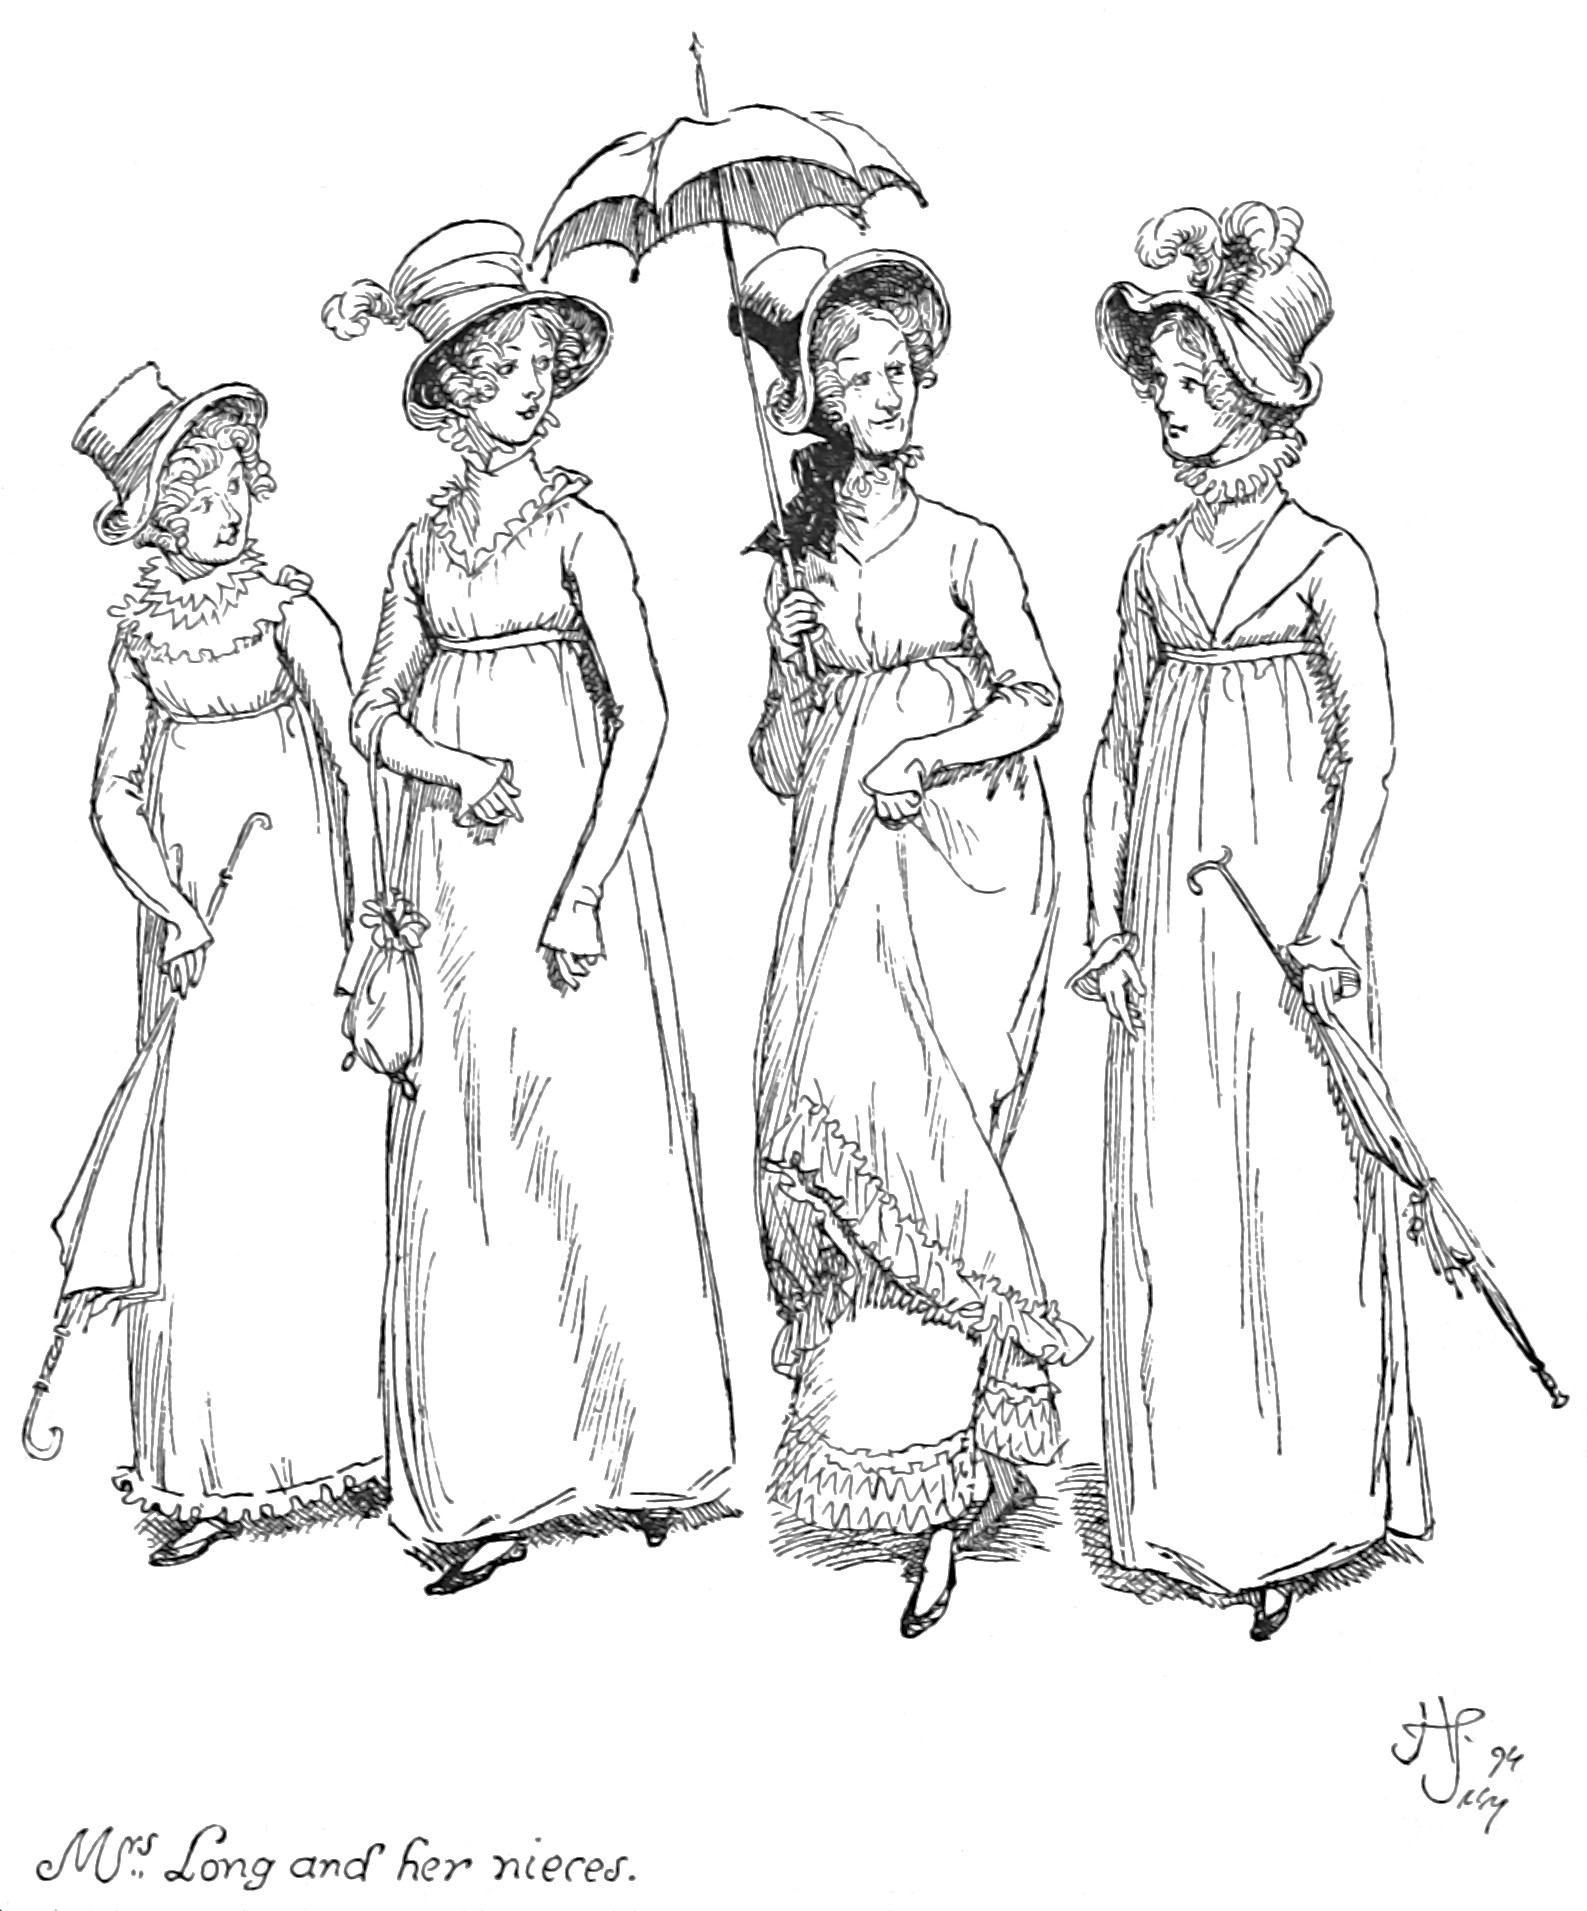
\includegraphics[width=.8\linewidth]{54nieces}
\captionlistentry{Mrs Long and her nieces}
\end{figure}

Mrs Bennet, in short, was in very great spirits: she had seen enough of Bingley's behaviour to Jane to be convinced that she would get him at last; and her expectations of advantage to her family, when in a happy humour, were so far beyond reason, that she was quite disappointed at not seeing him there again the next day, to make his proposals.

»It has been a very agreeable day,« said Miss Bennet to Elizabeth. »The party seemed so well selected, so suitable one with the other. I hope we may often meet again.«

Elizabeth smiled.

»Lizzy, you must not do so. You must not suspect me. It mortifies me. I assure you that I have now learnt to enjoy his conversation as an agreeable and sensible young man without having a wish beyond it. I am perfectly satisfied, from what his manners now are, that he never had any design of engaging my affection. It is only that he is blessed with greater sweetness of address, and a stronger desire of generally pleasing, than any other man.«

»You are very cruel,« said her sister, »you will not let me smile, and are provoking me to it every moment.«

»How hard it is in some cases to be believed! And how impossible in others! But why should you wish to persuade me that I feel more than I acknowledge?«

»That is a question which I hardly know how to answer. We all love to instruct, though we can teach only what is not worth knowing. Forgive me; and if you persist in indifference, do not make \textit{me} your confidante.«